\documentclass[11pt, letterpaper]{article}
\usepackage[letterpaper, margin=1in]{geometry}

\usepackage[hidelinks]{hyperref}
\usepackage{graphicx}
\usepackage{enumitem}

\begin{document}

\begin{titlepage}
  \begin{center}
      \vspace*{2cm}
      
      \fontsize{14}{14}\textbf{Jersey Number Recognition:} \\
      \vspace{0.1cm}
      \fontsize{14}{14}\textbf{Improving Pipeline Performance for the SoccerNet Challenge}
      
      \vspace{0.5cm}
      Presented by \\
      Riley Eaton, Aidan Elliott, Jerry Fan
      
      \vfill
      
      COSC 419/519: Deep Learning \\
      University of British Columbia \\
      Kelowna, BC \\
      April 8, 2025

  \end{center}
\end{titlepage}

% -------------------------- INTRODUCTION --------------------------
\clearpage
\section{Introduction}
The goal of the work presented in this report is to successfully identify the jersey numbers of soccer players via collections of video frames in image format. Each of these frames are represented with an image, and we will further refer to a collection of these images as tracklets. The full dataset is publicly available for the SoccerNet challenge, and is available on GitHub \cite{soccernet_repo}. Data analytics in sports have become increasingly present in the management and consumption of sports media. This has led to an increasing demand for robust player identification and tracking. Facial recognition has seen a significant improvement in recent history, however, video footage containing distance, occlusion, and orientation changes limit its usability in live identification. Nearly all broadcasted sporting events make use of jersey numbers so that officials, commentators, and spectators can identify and keep track of players in the game without needing to know their names. Since jersey numbers are typically large, unchanging, and have consistent patterns, determining them through modern deep learning techniques can be an accurate method of identifying players, though challenging. Employing such a system will lead to robust player recognition software, allowing sports organizations to improve the viewing experience for their fans. We aim to make this a possibility by introducing small, yet significant improvements on top of existing state-of-the-art pipelines which currently fall short of the accuracy required for such robust systems.


% -------------------------- LITERARY REVIEW --------------------------
\section{Literary Review}

Since Scene Text Recognition models are intended to identify text from an image, they present a unique opportunity to achieve inexpensive synthetic image generation. Bhargavi et al. \cite{bhargavi} used image generation to help identify Seattle Seahawks jersey numbers from practice videos. There was not a public dataset which fit their need to detect jersey numbers, so they decided to create their own. They did this by transforming jersey-like fonts that were similar to that of the Seahawks, to imitate the orientation changes that real jerseys experience in a live setting. They then superimposed this onto a random image to imitate background noise, as the pose detector won't be perfect in practice. By creating thousands of these images, they were able to fine-tune their model and improve the performance of the base CNN. The distribution of jersey numbers in a real setting are also highly imbalanced, as players have a variety of biases such as selecting single digit numbers, or digit pairs like 11, 22, etc. The synthetic dataset prepares more images with less-seen numbers to improve the model's ability to detect jersey numbers that are underrepresented in training data.

Koshkina and Elder's \cite{main_paper} introduce a comprehensive pipeline for detecting soccer jersey numbers in video tracklets as discussed. For each of the images within a tracklet, Koshkina and Elder fine-tune a binary CNN classifier based on ResNet34 to determine the frames that contain visibly legible numbers. Then, VITPose — a vision transformer — estimates the bounding box around the jersey number, and crops out the torso region. Finally, the scene text recognition model, PARSeq, is fine-tuned to predict the jersey numbers from the remaining images.

At the tracklet level, the image-level approach is extended further. Prior to the legibility classifier step, Centroid-ReID is used to filter the main subject. In particular, the system extracts a feature vector from each image in the tracklet using a pre-trained ReID network; then, it fits a Gaussian distribution to these features and removes any outlier images whose features are far from the mean, assuming those do not belong to the main subject. Here, only images which are visually similar to the main subject are kept for further processing. Then, a legibility classifier, pose estimation, and STR are implemented in order to detect and predict jersey numbers. The detection and localization using pose key points from ViTPose to crop the torso region. The STR model PARSeq is fine-tuned using real jersey numbers and used to predict numbers for each frame. The prediction model aggregates frame evaluation using both the heuristic method and the probabilistic method. Lastly, the aggregation of image-level prediction results is combined and assessed to generate the final prediction.

Koshkina uses both Hockey and Soccer datasets to test generalizability. Results indicate that the final accuracy of prediction is 91.4\% on hockey images and 87.4\% on soccer tracklets for the respective test sets \cite{main_paper}. This pipeline served as our baseline model, upon which we introduce our improvements.

Alternatively, Zhao et al. \cite{zhao_decoder} propose an approach to enhance scene text recognition (STR) by introducing Decoder Pre-training with Only Text (DPTR). Their method uses Contrastive Language-Image Pre-training (CLIP) to improve the STR model's performance.  The main goal of DPTR is to reduce the dependence on STR models' need for large amounts of labelled real images in the training steps. In Zhao's study, integrating DPTR with STR methods results in performance improvements. PARSeq, in particular, when combined with the DPTR technique, experiences a 1.6\% improvement in prediction accuracy over the baseline model \cite{zhao_decoder}.

CLIP is a model built by OpenAI; it learns to map text embeddings with images, allowing natural language prompts to be directly compared with images. Zhao's approach first involves performing text-to-embedding conversion. This allows the DPTR to use CLIP's text encoder to convert prompts into 512-dimensional embeddings, which serve as pseudo-visual features. Then, the CLIP image encoder is also used to simulate the variability found in actual image features. Additionally, random noise is applied to the image encoder features to prevent overfitting. The model proceeds with pre-training and fine-tuning steps by adding the offline random perturbation to the features generated with the CLIP text encoder. 

% -------------------------- SYSTEM DESIGN --------------------------
\section{System Design}

As mentioned, the design of our pipeline has been extended from that of Koshkina and Elder's \emph{General Framework for Jersey Number Recognition} \cite{main_paper}. Our improvements to the pipeline involve changing and fine tuning different parts of the models pipeline, however the general pipeline flow remains the same. Since any individual frame of video picked at random can be of poor quality or where a jersey number is occluded, it is better to use a tracklet of frames and consolidate a prediction based on all of them, which is the method implemented in this pipeline.

\subsection{Legibility and ViTpose}

In order to reduce the computation by inference on every frame in a list, it is easier to first identify models using a legibility classifier. Koshkina and Elder use a boolean output ResNet34 model to indicate whether the image is worth processing on. This step is important for broadcasters, as large computational costs limits the speed at which analytics can be provided to the fans. Any images in the tracklet deemed illegible by the model will be dropped from the remaining pipeline processes. Our initial plan was to dramatically increase the complexity of the model by increasing to ResNet 101, but once the immense time required for fine-tuning using this architecture was understood, we decided on the use of ResNet50 instead. We hypothesize that this deeper network will learn the more complex and abstract features associated with jersey numbers more accurately than the original ResNet34. 

The next step is to pass remaining images into a ViT Pose, a vision transformer which identifies the position a human body is in. The remaining images are still full sized containing copious amounts of noise, and we want to limit the space in which our number recognition model must derive a number from. This vision transformer can predict the shape in which the player is in, and return us a bounding box of the player's torso. Player jerseys are great for these models as their shirts are generally quite monotone in colour, and contrast with the background. The cropped output of the vision transformer will be passed on to our Scene Text Recognition (STR) model. It is of note that the group decided it was unnecessary to try and improve the pose model for our pipeline. In the examples we saw, the errors were clearly from poor legibility of the images rather than a poor bounding box. Even a theoretically perfect bounding box would not have produced any different results, so we happily left it alone.

\subsection{STR Model}

A scene text recognition model is able to output any text found in an image. Koshkina and Elder use PARSeq, a state of the art model \cite{parseq}. STR models are intended for generalized use at detecting many types of characters in many scenarios. However, our intended purpose for the STR is to exclusively identify numbers on players jerseys. Since our use case is far more nuanced, this is a great opportunity to fine-tune our model with more data. We intend to do this by using the same fine-tuning method as Koshkina and Elder, but with slight alterations.

We believe the biggest issue with the original pipeline architecture was the lack of unique data used to train the models. The dataset provided by SoccerNet may contain hundreds of thousands of images in the training set, however they combine to just 2853 tracklets \cite{soccernet_repo}. Training a complex deep learning model on 2853 examples is extremely small. To go along with this, many of these tracklets are from the same games and camera angles, further proneing the model to overfit certain attributes. In order to help create more data and fine tune the STR model, we employ similar practices to that presented in the work by Bhargavi et al., by creating a synthetic jersey dataset using python's Pillow library. Their paper was used to detect American football jerseys of a specific team, however the idea easily translates to any sport by simply changing fonts and colours of the numbers being generated. 

\subsubsection{Image Generation}

The dataset used by Bhargavi was not publicly available, so we created my own algorithm to generate the images. The algorithm first generates two random digits, and places them on a solid colour background. The Freshman font was used as it better mimics what a jersey number looks like. Each digit undergoes scaling, shearing, and rotation to mimic how a player's jersey will be transformed in a real image. Each transformation parameter follows a uniform distribution and is truncated to prevent any completely unreasonable results. A random level of Gaussian blue is also added to mimic the distance at which the camera is from the player. Since the VitPose will not create a perfect bounding box of the jersey, we place our synthetic jersey on top of a random image pulled from a subset of ImageNet mimic noise in the background. Any sort of multi-class image dataset would have probably sufficed, ImageNet was just a convenient diverse set of image classes.

With this algorithm, we can produce an entire dataset to train PARSeq. After some initial tests to make sure it was compatible, we created 100,000 images (~1000 images per digit) with a diverse set of positioning, transformations, and blurs. After this experiment, we also modified the algorithm to reduce the width of the jerseys so that the digits were far closer together and more resembled a jersey. We retrained this model using 10,000 of the new synthetic images followed by SoccerNet fine-tuning. An example of these images can be seen is Figure \ref{fig:synthetic_example}.

\begin{figure}
  \centering
  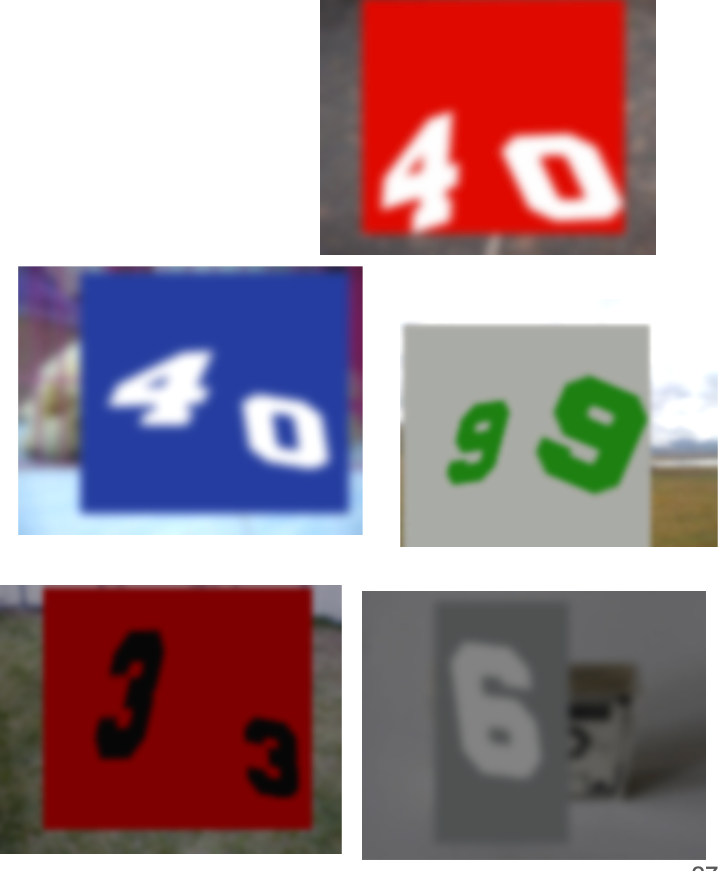
\includegraphics[width=0.5\linewidth]{img/synthetic_example.png}
  \caption{\label{fig:synthetic_example}\textit{Some example images from our synthetically generated dataset.}}
\end{figure}

\subsubsection{Training Precision}

When reviewing the source code of the original pipeline, it was apparent that the fine-tuning for PARSeq was hardware constrained. This is because not only did they specifically choose DDP as the training strategy — which is a dedicated method for utilizing multiple GPUs — but they also chose to use 16 bit mixed-precision training. This uses BF16 floating point numbers to reduce the amount of memory in training, but it comes with the downside of less accuracy. We decided that true 32 or 64 bit precision training would be beneficial to our model's performance, even if only slightly. This is primarily due to the fact higher precision arithmetic is less likely to round values to 0 when they are very small. This reduced rounding error leads to less gradient underflow, resulting in a more accurate model.

\subsubsection{CLIP Integration}

We previously discussed the similar work of Zhao et al. on the CLIP model for comparing natural language prompts directly with images. Although it would be beneficial to incorporate this work into our improved pipeline. Limited testing results show that pre-training only on natural language prompts without the offline random perturbation does not improve the pipeline performance. With this in mind, and due to the time-limited environment of our research, we decided not proceed with this integration, and this method is not included in our final results.

\subsection{Prediction Consolidation}

After each remaining image in the tracklet is individually passed through PARSeq and receives a result, all the predictions must be consolidated into one final result. Two distinct consolidation approaches were tested in Koshkina and Elder's work to perform tracklet-level predictions. The heuristic consolidation introduces two key measures: firstly, a tracklet is marked illegible if the total confidence score across all legible frames does not exceed a predefined threshold. Secondly, within a tracklet, if some images are predicted to contain double-digit numbers and others are predicted to contain single-digit numbers, the votes for single-digit numbers are down-weighted. Both strategies help to improve the overall tracklet prediction accuracy.

The probabilistic consolidation, on the other hand, considers the first and the second digit separately. A vector containing digits 0-9 is used to predict the probability of each digit for each position of the jersey number. A bias of 39\%, representing the ratio of single-digit jerseys in the dataset, was incorporated. Then, a standard temperature scaling algorithm was applied to calibrate the output probabilities to reduce overconfidence. The final prediction of each digit was made by combining the adjusted probabilities across all legible frames.

Koshkina and Elder indicated that the heuristic consolidation overperformed the probabilistic consolidation, achieving a 2.23\% higher accuracy in their final prediction results \cite{main_paper}. Thus, the heuristic consolidation approach was chosen in the original pipeline. This is left relatively unchanged for our final pipeline. However, as discuss in section 5.1, a bug we found that caused the pipeline to output -1 despite the STR model being very confident in detecting a number.

% -------------------------- RESULTS --------------------------
\section{Results}

\subsection{Initial Replication Results}

Our initial results for replicating the pipeline used the pre-trained model checkpoints provided in Koshkina and Elder's GitHub repository \cite{original_pipeline_repo}. These resulted in a slight decrease accuracy of 0.75\% on the test set, for the entire pipeline. After this, we decided to re-fine-tune the STR and legibility models by running the training procedure provided. However, there were many hurdles in getting the training to run. Initially the training script was riddled with errors, mostly due to outdated libraries. Additionally, the code was developed with a linux development environment in mind (filepaths specifically). This was an issue because one of our group members who has access to a significant GPU for training train, uses Windows. It took some time to iteratively solve these issues, but we were eventually able to get the training to successfully complete. Below are tables illustrating our inference results, and the required time for each step of training, respectively: 

\begin{center}
  \begin{tabular}{|l|c|}
    \hline
    \textbf{Method} & \textbf{Test Accuracy} \\
    \hline
    Orignal (out-of-the-box)  & 80.51\% \\
    Fine-tune on Hockey       & 83.90\% \\
    Fine-tune on SoccerNet    & 87.45\%  \\
    \hline
    Our initial run & 86.70\%  \\
    \textbf{Our fine-tune on SoccerNet} & \textbf{87.60\%}  \\
    \hline
  \end{tabular}
\end{center}
\begin{center}
  \begin{tabular}{|l|c|c|c|}
    \hline
    \textbf{Training Task} & \textbf{Epochs} & \textbf{Final Loss} & \textbf{Training Time} \\
    \hline
    Hockey legibility classifier                      & 10 & 0.001 & $<$ 1 min \\
    Soccer legibility classifier (using weak labels)  & 10 & 0.062 & 2 hours, 25 mins \\
    Fine-tune PARSeq (STR) on SoccerNet               & 25 & 0.0139 & 1 hour, 51 mins \\
    \hline
    Total training time & - & - & \textbf{4 hours, 16 mins}  \\
    \hline
  \end{tabular}
\end{center}

This small improvement of 0.15\% in model performance from the original paper after our fine-tuning is likely due to updated libraries such as CUDA, and not truly significant.

After this, we also noticed there was no mention in the original paper of fine-tuning the STR model on both SoccerNet and Hockey image datasets. We decided to try this experiment to see if the Hockey jerseys could improve PARSeq's performance on SoccerNet. Unfortunately, it led to a decrease of 0.81\% in performance, down to 86.79\% accuracy on the test set. We believe this decrease was caused by the very distinct jersey number features present in the two datasets.

\subsection{Synthetic Generation Results}

The first iteration of our testing on the synthetic dataset involved a fine-tune of PARSeq on 100,000 images before being fine-tuned again on SoccerNet. The result was rather disappointing, reducing test accuracy by 0.32\% to 87.28\%. This was not a significant decrease, but still did not improve the results very much. After updating the generation algorithm to include more noise, brightness and color changes, and bringing the digits closer together, we generated another 10,000 images. A new model was trained on these images then once again SoccerNet. These results came out worse, decreasing 0.92\% when compared to our best model. The paper our method is based on used 400,000 images to train their model, so more images were likely needed to produce better results. Unfortunately, we were restricted by the limited time available, and were not able to generate that many images.

\subsection{PARSeq64 Results}

Surprisingly, the most significant improvements to the pipeline were realized using true 64 bit precision training when fine-tuning PARSeq on the SoccerNet dataset. We call the output model (checkpoint) of this fine-tuning, PARSeq64. This model was trained for 15 epochs, and achieved a test accuracy of 88.69\% on the test set, and 86.04\% on the challenge set. This is a very impressive improvement over the original pipeline's accuracy, especially on the challenge set, being able to accurately predict 6.73\% more jersey numbers correctly. The results of our PARSeq64 model compared to the work from Koshkina and Elder, and previous works can be seen in table below, which is amended from the original paper \cite{main_paper}:

\begin{center}
  \begin{tabular}{|l|c|c|}
    \hline
    \textbf{Method} & \textbf{Test Accuracy} & \textbf{Challenge Accuracy} \\
    \hline
    Gerke et al.  & 32.57\% & 35.79\% \\
    Vats et al.  & 46.73\% & 49.88\% \\
    Li et al.    & 47.85\% & 50.60\% \\
    Vats et al.  & 52.91\% & 58.45\% \\
    Balaji et al. & 68.53\% & 73.77\% \\
    \hline
    Koshkina and Elder & 87.45\% & 79.31\% \\
    \hline
    \textbf{Ours} & \textbf{88.69\%} & \textbf{86.04\%} \\
    \hline
  \end{tabular}
\end{center}

\begin{center}
  \textit{The above test set accuracy of our PARSeq64 model has been validated by EvalAI, and the output file for the submission is publicly available \underline{\href{https://evalai.s3.amazonaws.com/media/submission_files/submission_503522/62c51842-1475-414e-94cf-373e5d51920e.txt}{at this link}}. As well, the output file for our challenge set evaluation using PARSeq64 is available \underline{\href{https://evalai.s3.amazonaws.com/media/submission_files/submission_503523/1b5b6636-a642-4490-9bd8-67120830fe24.txt}{at this link}}}
\end{center}

Although these results are impressive, it is important to note that the training took significantly longer because of this increase in precision. Averaged over all epochs, the original 16 bit mixed precision training took 4.5 minutes per epoch on our NVIDIA 4070 GPU, while the true 64 bit training increased to 45 minutes per epoch. This 10 times slower training time is a significant drawback, however, it is slightly mitigated by requiring fewer total epochs for convergence. The original model saw its best performance at 25 epochs, while our PARSeq64 model converged at 15 epochs. This resulted in a total time increase for training of 6 times the original pipeline. Given the total training time was just over 11 hours, this was still acceptable for us given the compelling increase in performance. 

To summarize our results, the final accuracy of our most critical tests can be compared to that of the original pipeline in the following table, sorted in ascending order of accuracy:

\begin{center}
  \begin{tabular}{|l|c|c|}
    \hline
    \textbf{Method} & \textbf{Test Accuracy} & \textbf{Challenge Accuracy} \\
    \hline
    Our initial replication (out-of-the-box models) & 86.70\% & - \\
    Our SoccerNet and Hockey fine-tune & 86.79\% & - \\
    Our synthetic image fine-tune & 87.28\% & - \\
    \textbf{Koshkina and Elder} & \textbf{87.45\%} & \textbf{79.31\%} \\
    Our first local fine-tune & 87.60\% & - \\
    \textbf{Our PARSeq64 fine-tune} & \textbf{88.69\%} & \textbf{86.04\%} \\
    \hline
    \end{tabular}
\end{center}

% -------------------------- DISCUSSION --------------------------
\section{Discussion}

\subsection{Prediction Consolidation Oversight}

When analyzing the performance of our PARSeq64 model, we noticed an alarming issue with one of our tracklets. In tracklet 111 of SoccerNet's test set, we noticed that our STR model predicted the jersey to be number 34 with 99.7\% accuracy. However, after consolidation of predictions, it outputted -1! After some digging, we realized that the authors included a check that increases the weight for two-digit numbers. This is a very rational decision, as a common issue with predicting jersey numbers occurs when a player is contorted such that only one of two digits are visible in the camera, producing a one digit output. Therefore, if half the frames where only one digit is visible and the other half show both, the prediction consolidation will still successfully pick the double-digit number. However, the authors failed to account for the option when only one or two frames are deemed eligible before being passed into the prediction consolidation.

Each frame's confidence is multiplied by 0.61 or 0.39 for double digits and single digits, respectively. Most scenarios deem many frames legible, so this is not generally an issue. The prediction consolidation sums all the weights of frames that share the same prediction, and outputs the prediction with the highest summed weight. However, if the highest weight is less than one, it will be deemed illegible and output -1. Since the most weight a single frame can have is 0.61, tracklet 111 will always output -1 no matter how confident it is in that one frame. In tracklet 111's case, only one frame is considered legible, and 0.997 * 0.61 is less than one thus inferred to be an illegible jersey by our prediction consolidation. 

To fix this issue, we created a bypass to be used when there was only one unique prediction output and its confidence was greater than 0.9. The chosen cutoff is arbitrary and we acknowledge that altering it could be experimented with. After re-inferencing the model we found an immediate improvement from 88.69\% to 88.85\% on the test set. The bypass fixed the prediction for track 111, as well as two other cases in the test set. Since examining the test set to get better accuracy may be considered cheating to some degree, we do not consider this an official increase in performance. However, it was an interesting discovery that demonstrates there is more performance to be gained in the prediction consolidation.

\subsection{Why ResNet50 Didn't Improve}

After training our ResNet50 model on the same number of epochs as ResNet34, we quickly noticed the performance was lower. Since ResNet50 is a deeper network, we believed this decrease was simply due to slower convergence, so we decided to train it for more epochs. After doing so, ResNet50 converged to a similar accuracy as ResNet34. However, we noticed that as it began to no longer see gains in validation accuracy, the accuracy began to fluctuate significantly. We retrained the model using an optimizer that reduces the learning rate if a plateau or decrease in validation accuracy is detected for 2 consecutive epochs, called ReduceLROnPlateau. This still resulted in ResNet50 converging to a very similar accuracy as ResNet34, which stagnated after 8 epochs as seen in Figure \ref{fig:Resnet_Validation_Accuracy_Comparison}. Additionally, we observed the train set quickly became asymptotic, reaching 95\% within 3 epochs, and 99\% by epoch 10, illustrating that this classifier is very likely overfitting. Even more importantly, there is a large disparity that remains for every training epoch, between the test and validation accuracy which can be seen in Figure \ref{fig:Resnet_Validation_vs_Test_Accuracy}, further proving our hypothesis of overfitting. This experiment led us to the conclusion that in order for a deeper network to be trained for this problem, more data with even more diverse classes mis necessary to see any performance gains against the smaller, ResNet34 architecture.

\begin{figure}
  \centering
  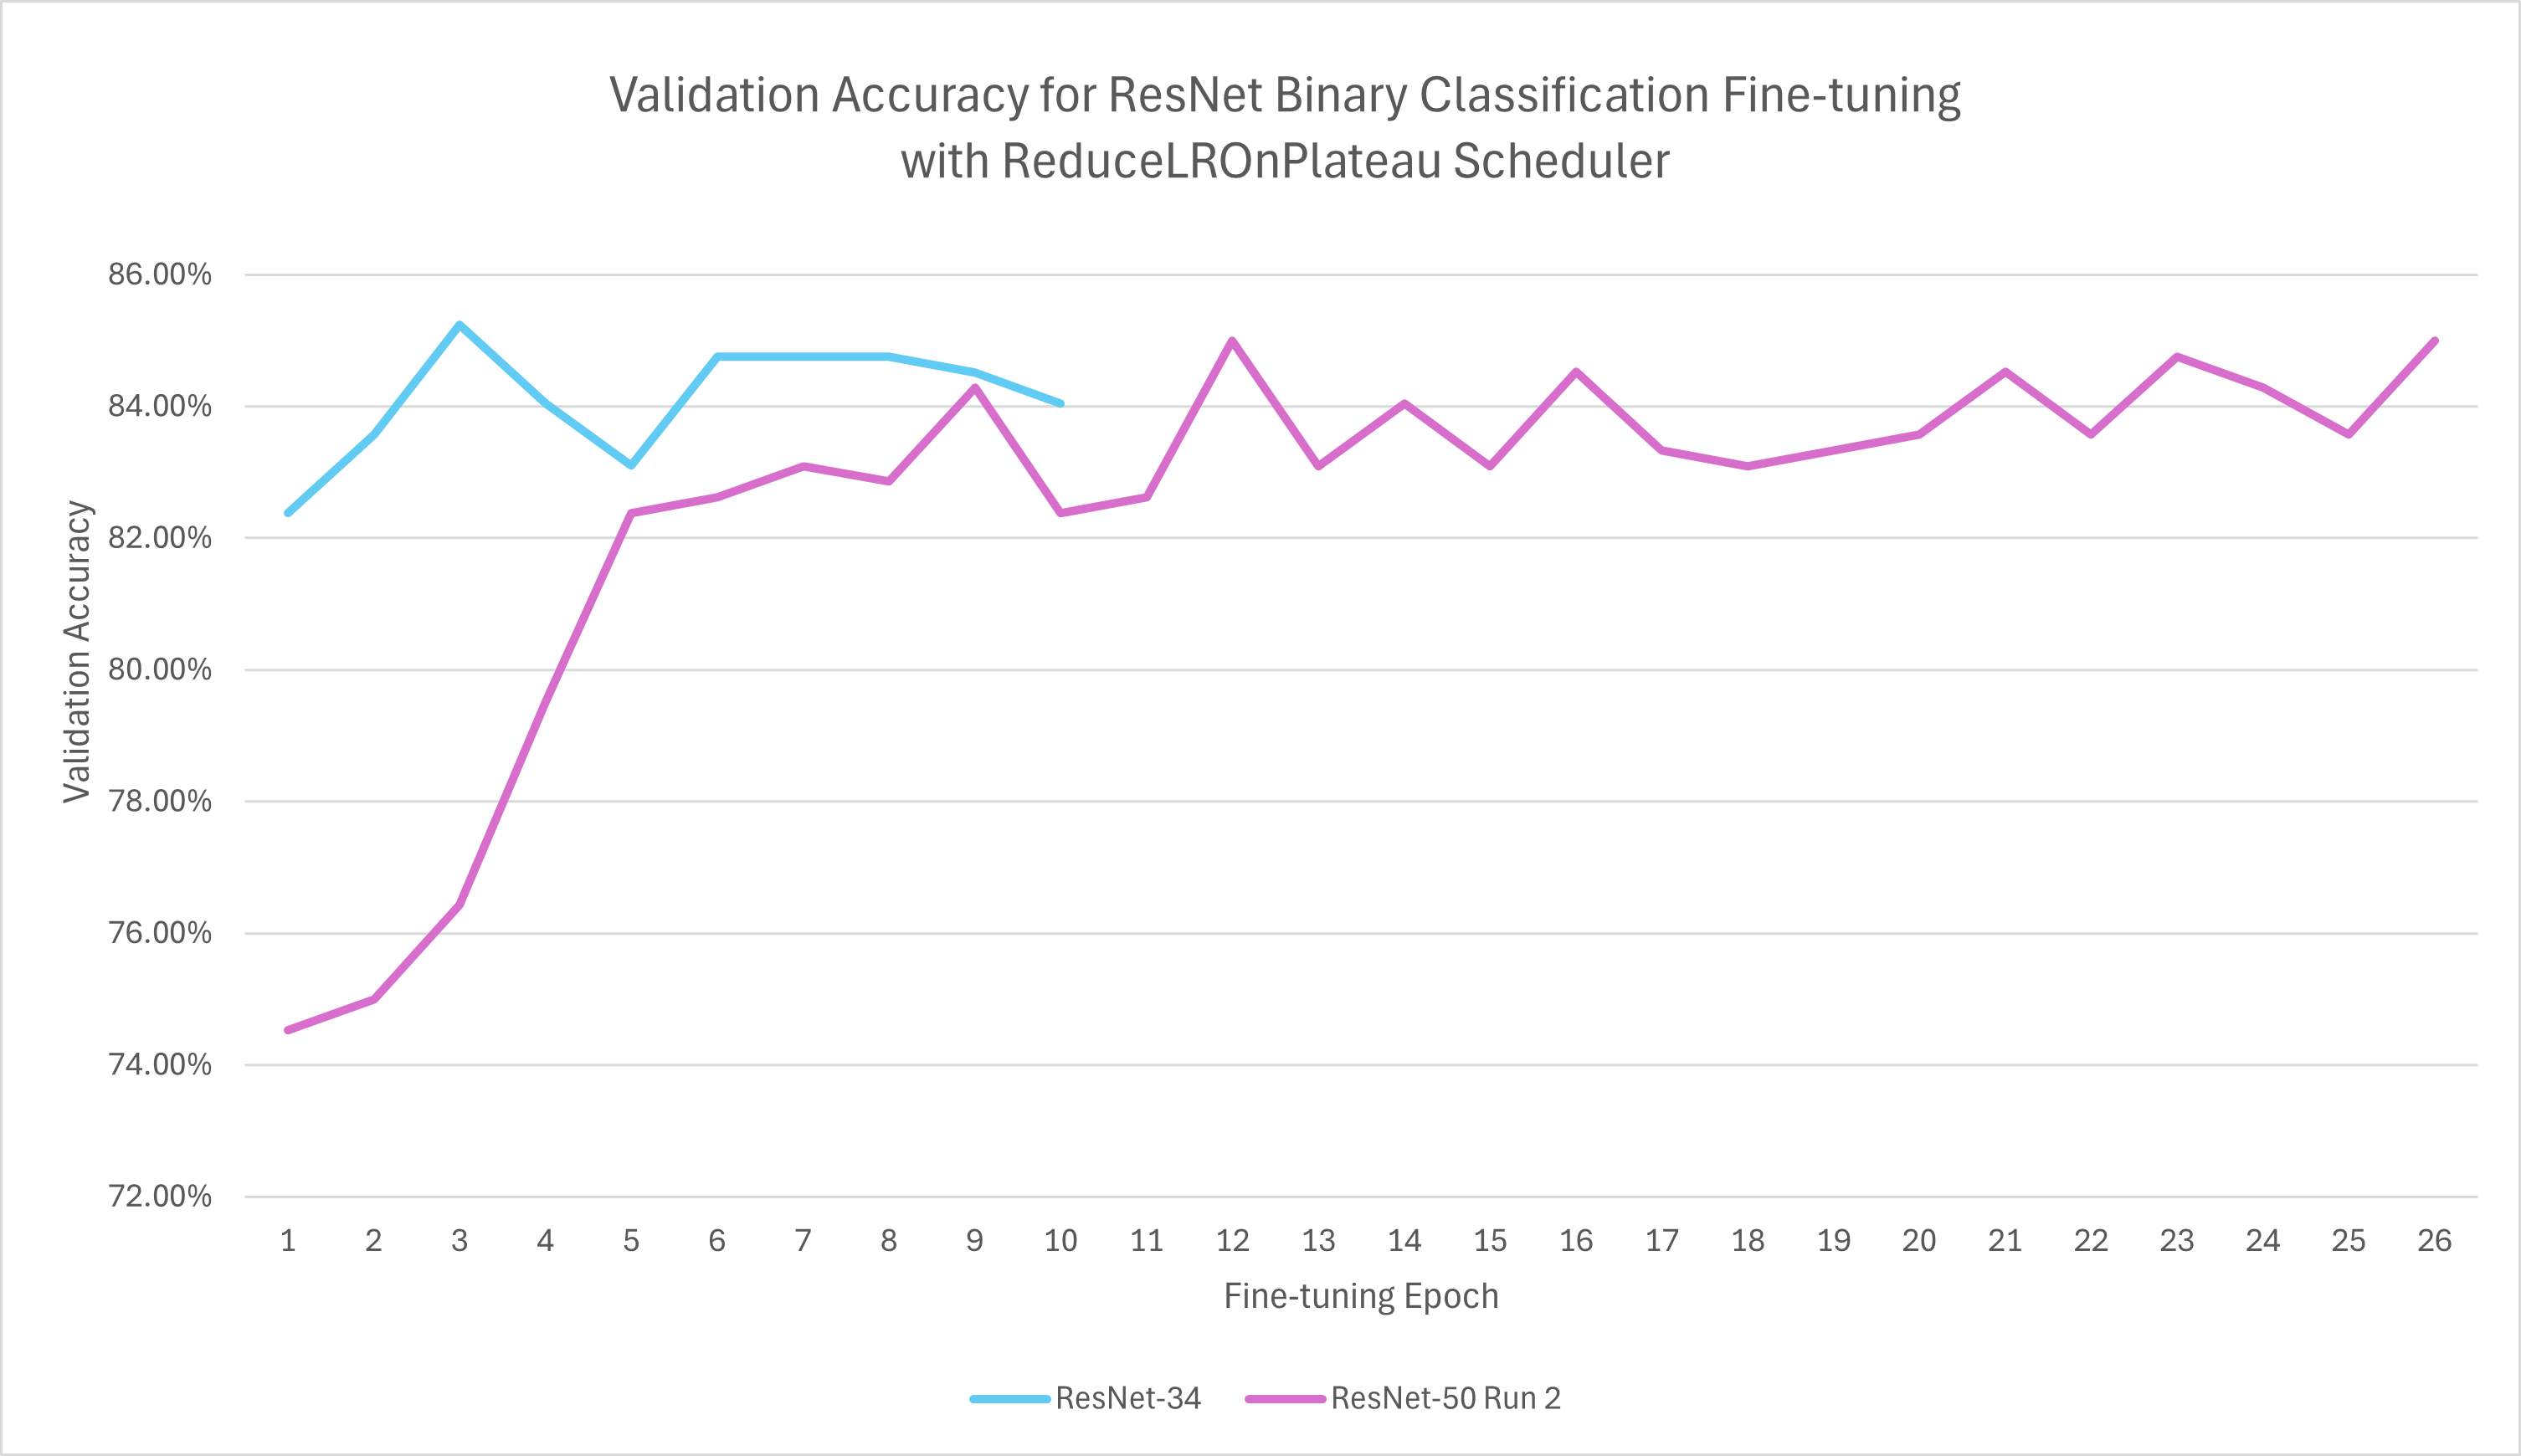
\includegraphics[width=0.8\linewidth]{../results/Resnet_Validation_Accuracy_Comparison_ReduceLROnPlateau.png}
  \caption{\label{fig:Resnet_Validation_Accuracy_Comparison}\textit{Test vs validation accuracy comparison when fine-tuning ResNet50 over 25 epochs for binary classification on the SoccerNet dataset. The early plateau with little long term improvement is a sign of overfitting.}}
\end{figure}

\begin{figure}
  \centering
  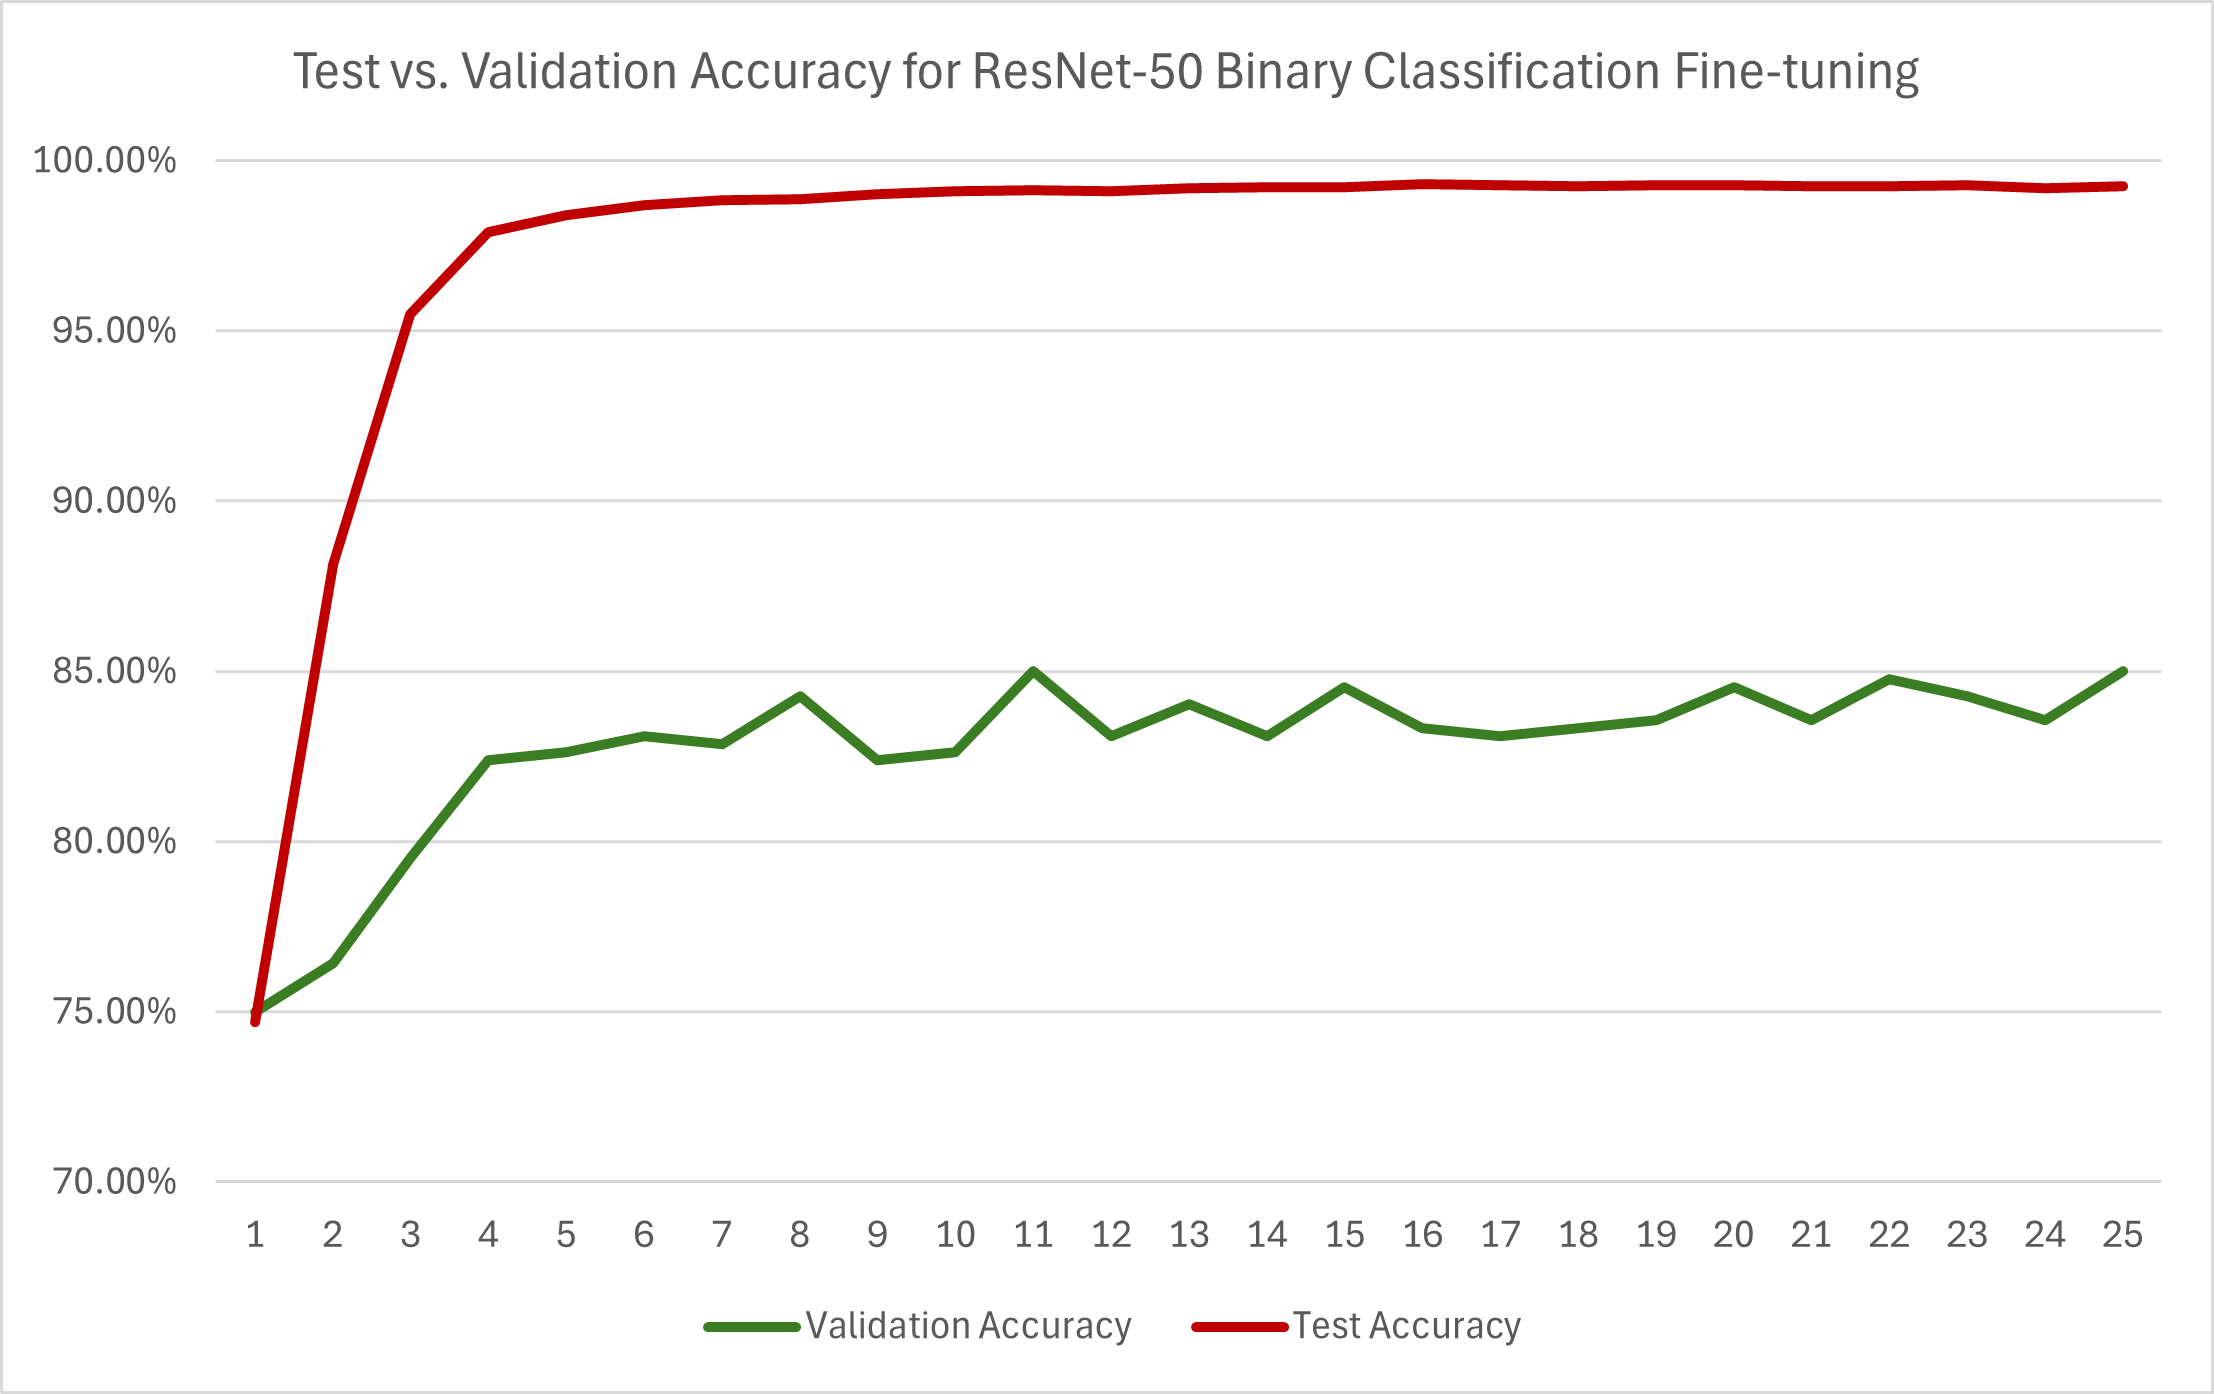
\includegraphics[width=0.8\linewidth]{../results/Resnet_Validation_vs_Test_Accuracy_Comparison.png}
  \caption{\label{fig:Resnet_Validation_vs_Test_Accuracy}\textit{Test vs validation accuracy comparison when fine-tuning ResNet50 over 25 epochs for binary classification on the SoccerNet dataset. The disparity between the two — especially early in fine-tuning — is a sign of early overfitting.}}
\end{figure}

\subsection{Legibility Performance Bottleneck}

Upon analyzing the incorrectly predicted tracklets, a trend appears. Of the tracklets which our PARSeq64 pipeline predicts wrong in the test set, roughly 75\% of them have either a true value of -1, or a predicted value of -1. Therefore, any improvements to the number recognition of the STR model would have realize limited performance gains for this dataset. Since training is done on weakly labelled data using a legibility classifier fine-tuned on hockey jerseys, there are certainly some that are incorrectly labelled. This may be a cause of reduced performance that should be investigated further. If we had a very large amount of data, an occasional incorrect label would not change training performance significantly. However, the amount of data available in SoccerNet to fine-tune is already somewhat limited, and are not diverse enough to create a truly robust model (same games, cameras, etc.). Due to this, we believe the legibility classifier implantation using ResNet34 and ResNet50 will always overfit in this case, and therefore not be able to generalize well on different soccer datasets. Had we noticed this pattern in the data sooner, we would likely have shifted our focus to improving the legibility classifier in other ways.

\subsection{Why Synthetic Jerseys Failed}

Overall, training on the synthetically generated jersey dataset did not improve the accuracy of the STR model. It instead reduced performance by roughly 1\%. There are plenty of potential reasons why the dataset did not improve performance like it did in Bhargavi's paper. We suspect this is mainly due to more randomness in the scaling and level of noise required. We discovered later in our research that PARSeq was already somewhat accurate in predicting numbers at this level of distortion, so the images did not have anything useful for the model learn, ultimately contributing features that only served as distractions. Additionally, in extreme cases, the random affine transformation caused the number to be cut off from the jersey, effectively causing the synthetic image to be mislabelled. This occurred in a small subset of the synthetic dataset, but still enough to cause potential issues.

Considering the conversation in 5.3, it is important to note that the majority of errors made by PARSeq are from tracklets which either have predicted -1, or have a label of -1. This means that improvements made to the STR model can only be realized to a degree, as incorrectly labelled images as illegible do not even get assessed by it. Also, it is important to note how imbalanced the dataset is. The majority of jerseys are biased towards single digit, low double digits (10-20), or repeated digits (i.e 55, 66). There simply are not many players who want to have “72” or “89” on the back of their jersey, and the dataset would likely contain at most 2 to 3 tracklets for these numbers. Also, this dataset is not comprised of enough games to provide a breadth of examples for many possible numbers. Using synthetic jerseys to create more examples can help the model generalize for less frequent numbers.

% -------------------------- FUTURE WORK --------------------------
\section{Future Work}

In future efforts to improve this jersey number recognition pipeline, we believe that the most important step is to improve the legibility classifier. This initial and crucial step in the pipeline has proven to be a significant area for improvement, and if it is not accurate, the rest of the pipeline will not be able to produce any better results. As discussed, using a larger dataset of soccer jerseys, with more diverse classes (number combinations, jersey colors, jersey patterns, background variations, etc.) would allow a fine-tuned model to learn more critical features, allowing it to ultimately improve in more complex scenarios.

We had also previously mentioned the notion that in a real setting, the distribution of numbers on player jerseys will not be equally weighted for all possible numbers (0 through 99). The reasons for this branch out into the field of psychology, and cannot be effectively discussed here. However, if we were aware of the true nature of this distribution, synthetic datasets could be created that are more representative of the real world, likely leading to increased performance in real settings.

Another interesting avenue of research we explored was using a Stable Diffusion image generation model to create a synthetic dataset for fine-tuning. Some basic experimentation showed that simple prompt engineering could create a solid example for a model to train on. The example in Figure \ref{fig:gemini_jersey} would undoubtedly provide more detail for the model to learn from, when compared to a those from a pseudo-random image generator such as the one we developed. Our result leads us to believe that with some experimental prompt engineering and a state-of-the-art transformer-based image generation model, an entire dataset could be created to further fine-tune models within the pipeline. However, this does bring with it a plethora of other issues such as the bias of the generation model, but with generative AI getting better each day, the use of these synthetic images to train other prediction models will certainly become a reality.

\begin{figure}
  \centering
  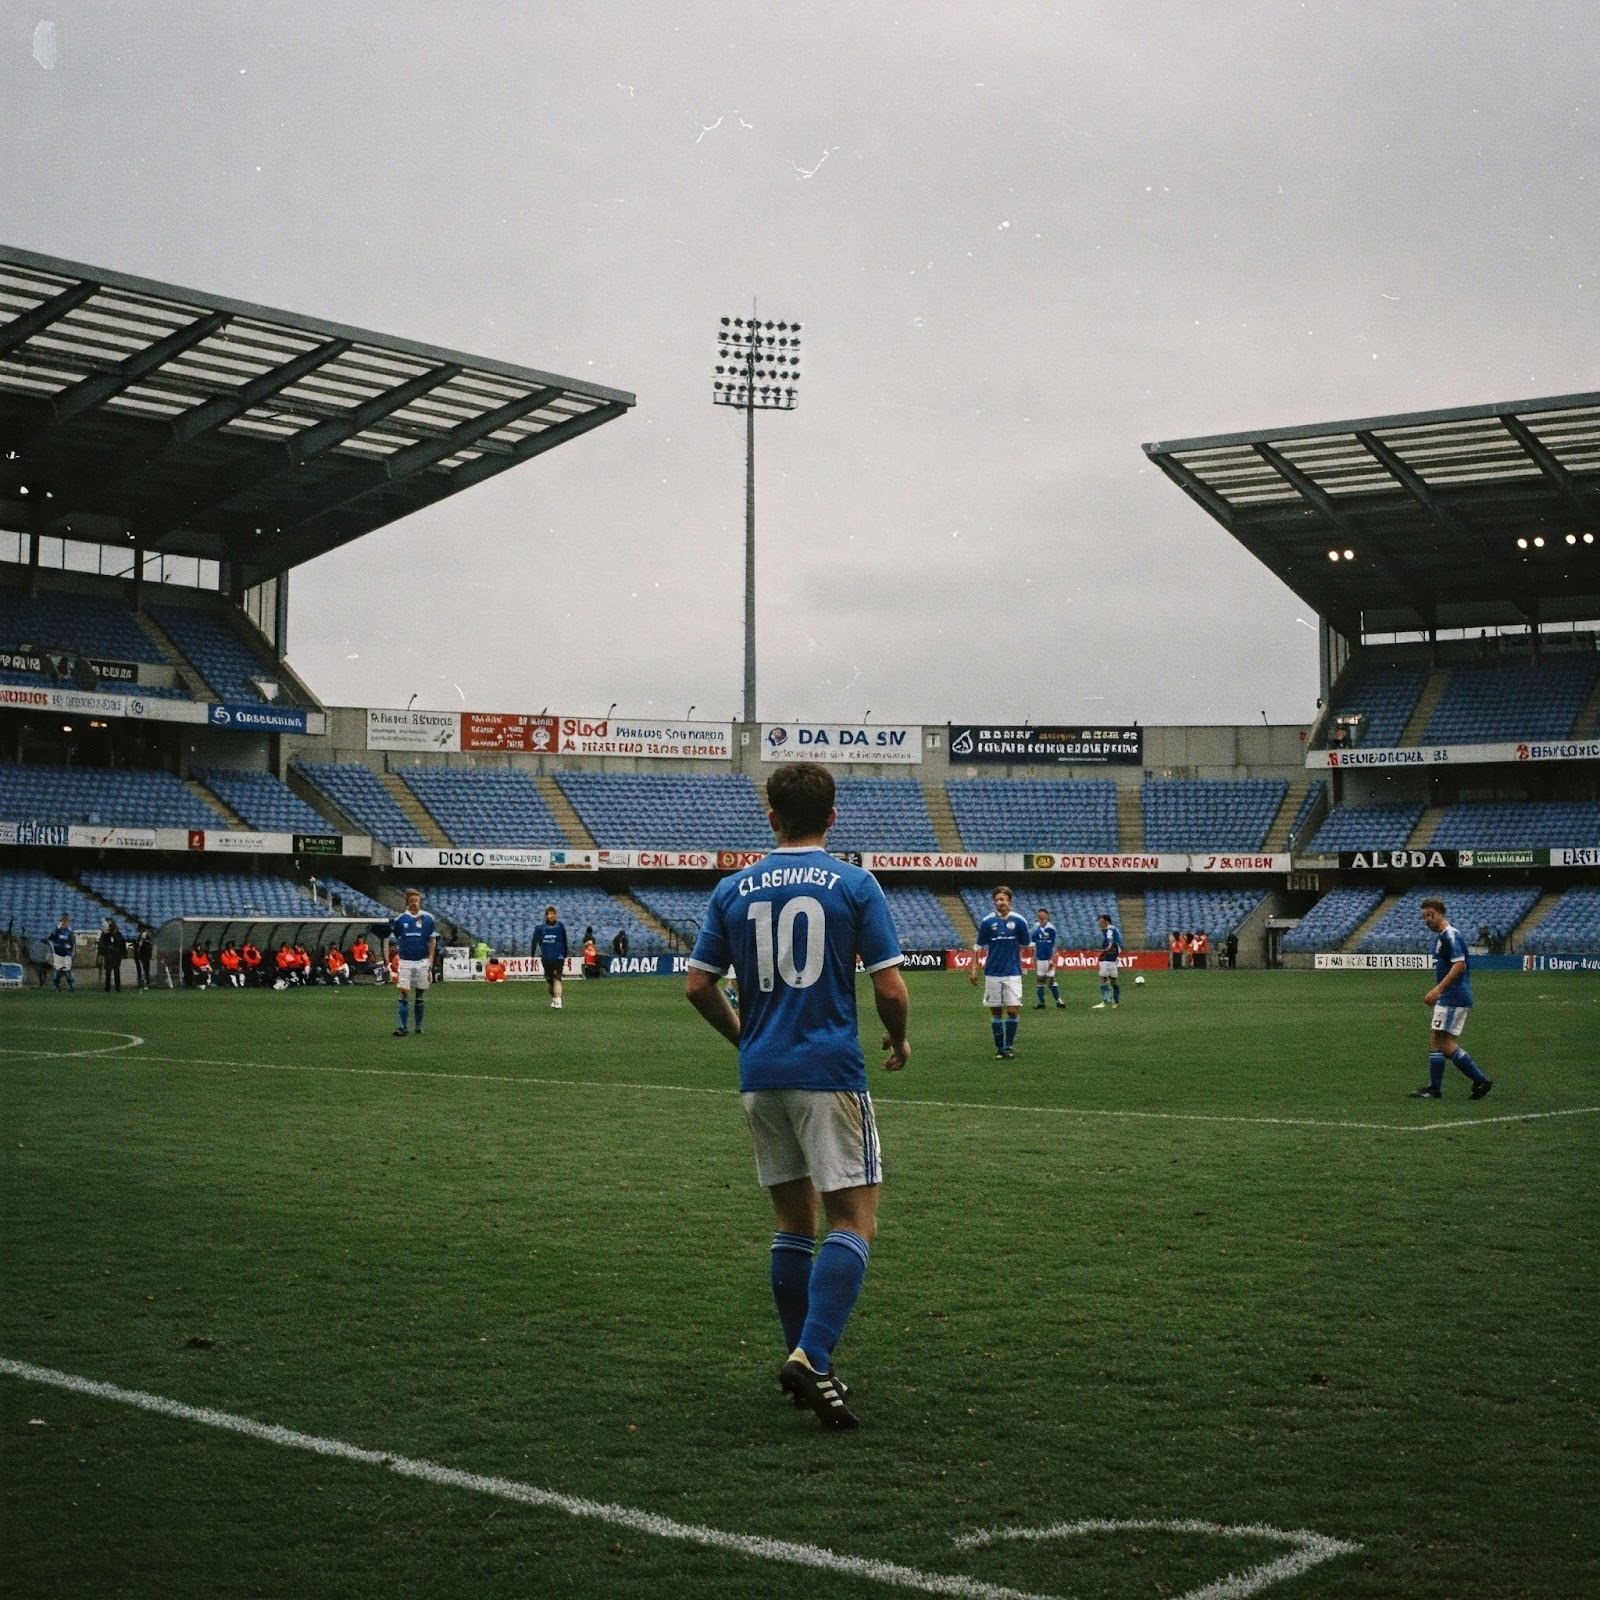
\includegraphics[width=0.5\linewidth]{img/gemini_jersey.jpg}
  \caption{\label{fig:gemini_jersey}\textit{Google Gemini result for the prompt: “Create me an image of a soccer player where you can see the back of his jersey and his jersey number. He needs to be from a distance and in a stadium”}}
\end{figure}

% -------------------------- REFERENCES --------------------------

\clearpage
\bibliographystyle{IEEEtran}
\bibliography{refs}

\end{document}